\documentclass[11pt, english, fleqn, DIV=15, headinclude, BCOR=2cm]{scrreprt}

\usepackage[
    color,
    bibatend,
]{../../header}

\graphicspath{{./}{../Figures/}}

\usepackage{needspace}

\usepackage{mathtools}
\usepackage{listings}

\lstset{
    basicstyle=\small\ttfamily,
}

\hypersetup{
    pdftitle=
}

\newcommand\mot{\textsc{mot}}

\usepackage{longtable}
\usepackage{subcaption}

\usepackage[all]{nowidow}

\subject{Lab report}
\title{Optical frequency doubling}
\subtitle{Experiment A245 -- Universität Bonn}
\author{%
    Martin Ueding \\
    \small{\href{mailto:mu@martin-ueding.de}{mu@martin-ueding.de}}
    \and
    Lino Lemmer \\
    \small{\href{mailto:l2@uni-bonn.de}{l2@uni-bonn.de}}
}

\date{\daterange{2016-05-23}{2016-05-24}}

\publishers{Tutor: Gautam Ramola}

\begin{document}

\maketitle

\begin{abstract}
\end{abstract}

\tableofcontents

\chapter*{Permission to upload}

I, Martin Ueding, would like to scan and upload this lab report with your
corrections to my website \href{http://martin-ueding.de}{martin-ueding.de}.
There, the original lab report as well as the reviewed one will be licensed
under the “\href{http://creativecommons.org/licenses/by-sa/4.0/}{Creative
Commons Attribution-ShareAlike 4.0 International License}”. Is that okay with
you?

Yes $\Box$ \hspace{2cm} No $\Box$

\chapter{Theory}


\section{Generation of hamonics}

\section{Birefringence}

\subsection{Retarder plates}

\section{Phase matching}

\section{Gaussian beams}

\subsection{Rayleigh length}

\section{Wavelength measurement}

\subsection{Gratings}

\subsection{Michelson interferometer}

\section{Coherence}

\subsection{Coherence length}

\section{Diode laser}
\label{sec:diode_laser}

% TODO Describe elliptical beam shape.

\chapter{Conduction and analysis}

\section{Diode laser classification}

First we want to classify the Laser diode at hand. We have a diode laser which
is mounted behind a safety shutter. One of the characteristics of a diode laser
is the elliptical beam shape as described in Section~\ref{sec:diode_laser}
already. Therefore our setup includes a pair of prisms in order to get a
circular beam cross section. The whole setup including the power meter is shown
in Figure~\ref{fig:fig-1}.

\begin{figure}
    \centering
    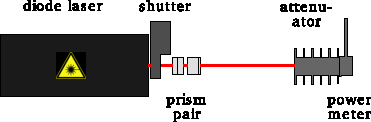
\includegraphics{fig-1}
    \caption{%
        Setup for characterizing the diode laser. Taken from the manual.
    }
    \label{fig:fig-1}
\end{figure}

For measuring the power we just dump the whole beam into a power meter. Since
the power meter become non-linear beyond \SI{20}{\milli\watt} we use an
attenuator in front of it. This will take away a certain fraction of the beam
and allow us to measure higher intensities. The attenuator has to be calibrated
first with small beam powers to allow for a comparison.

% TODO Measure up to 280 mA.
% TODO Measure background.
% TODO Calibrate attenuator.

\subsection{Injection current}

% TODO Plot output versus current.

\subsection{Threshold current}

% TODO Extract threshold.

\subsection{Quantum efficiency}

% TODO Compute differential slope efficiency.
% TODO Compute quantum efficiency from slope.

\subsection{Variable attenuator}
\label{sec:variable_attenuator}

The laser might experience \emph{mode hops} when we adjust the current.
Therefore we do not want to adjust laser power by the current during our
adjustment. We rather want to have an optical way to adjust the beam power. For
this we will use a polarizing beam splitter and a $\lambda/2$-plate in front of
that. By adjusting the polarization of the beam going into the polarizing
splitter we can select the portion of the power advancing to the next parts in
our setup. We extend out setup with a plate and splitter like shown in
Figure~\ref{fig:fig-2}.

\begin{figure}
    \centering
    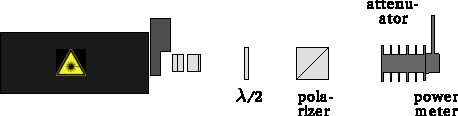
\includegraphics{fig-2}
    \caption{%
        %
    }
    \label{fig:fig-2}
\end{figure}

We must obtain a relation of retarder plate angle and output power to use this
later on. There is only one power meter and we want to measure the powers of
both the fundamental and harmonic beam at the same time. We take power
measurements of the fundamental beam in \SI{2.5}{\degree} steps of the retarder
plate.

% TODO Measure power depending on the retarder plate angle.

We expect to see a $\cos^2$ profile, perhaps with a constant offset.

% TODO Fit data.

\subsubsection{Extinction ratio}

% TODO Determine extinction ratio.

\section{Harmonic power}

Now we have the power measurement calibrated. We can determine the power in the
fundamental beam from the angle of the retarder plate. Our setup is extended
with the non-linear crystal and a filter as shown in Figure~\ref{fig:fig-4}.
The blue filter is needed to get rid of the fundamental wave, we only want to
measure the power of the harmonic wave here.

\begin{figure}
    \centering
    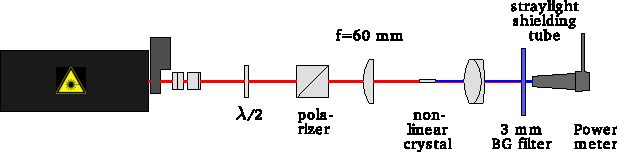
\includegraphics{fig-4}
    \caption{%
        %
    }
    \label{fig:fig-4}
\end{figure}

The crystal used here is a $\mathrm{KNbO_3}$ crystal. It has a cross section of
\SI{2}{\milli\meter} times \SI{1.8}{\milli\meter}. It is cut along the b-axis
and has a length of \SI{5}{\milli\meter}. The end faces are coating to avoid
reflections at \SI{987}{\nano\meter} and \SI{494}{\nano\meter}.\footnote{This
information is given on page~6 of the manual.}

% TODO Write about adjustment.

\subsection{Output power optimization}

With the rough optical setup in place we can insert the crystal and optimize
for maximum harmonic power. We slowly heat up the crystal to \SI{36}{\celsius}.
Then we slide it into the focus of our setup.

% TODO Check with paper behind the crystal that one can see something.

The blue harmonic light is focused with an achromatic lens and filtered with an
\SI{3}{\milli\meter} BG40 glass filter. From Figure~3 of the manual we estimate
a total transmission coefficient of \num{0.9} at \SI{494}{\nano\meter}. For the
unwanted fundamental wave we have a transmission coefficient of around
$10^{-2.3} = 0.005$.

% TODO Think about the effect of the fundamental wave in our measurement here.

We slightly move the crystal to optimize the output power.

% TODO Compute beam waist.
% TODO Compute Rayleigh length.
% TODO Determine the fulfillment of the Boyd-Kleinman condition.
% TODO Determine optimal focal length.

\subsection{Crystal temperature dependence}

Since the index of refraction is temperature depending in our crystal material
we want to measure the temperature dependence. First we cool down to
\SI{27}{\degree} in steps of \SI{0.5}{\celsius} and then heat up to
\SI{40}{\celsius} in steps of \SI{0.2}{\celsius}.

% TODO Take measurements of power and background at each temperature.

% TODO Plot data such that sinc shape can be seen.
% TODO Try to fit a sinc function.
% TODO Explain why the curve could be asymmetric.

Now that we know the optimal temperature for the crystal, we slowly tune the
temperature to this optimal setting.

\subsection{Input power dependence}

The output power must depend on the input power. As we have calibrated in
Section~\ref{sec:variable_attenuator}, we can choose an input power by rotating
the retarder plate in front of the splitter. We measure the output power while
adjusting the angle of the retarder plate.

% TODO Table with measurements.

% TODO Plot output power versus input power.
% TODO Determine expected relationship.
% TODO Fit model to data.
% TODO Extract frequency doubling efficiency.

\subsection{Input polarization dependence}

By taking out the polarizing beam splitter we can freely adjust the linear
polarization of the light that goes into the crystal. We take a set of
measurements of the output power with different angles of the retarder plate.

% TODO Table with measurements.

% TODO Plot.
% TODO What do we expect for type 1 and type 2?
% TODO Fit the data.
% TODO Are the fit parameters sensible?

\section{Wavelength comparison}

As this experiment is titled \emph{frequency doubling} we except that the
frequency of the incident beam has doubled pretty much exactly. In the
following parts we will compare the two wavelengths with each other and
determine how exact the doubling actually is.

\subsection{Grating}

The first and quick method is using a grating to have a wavelength dependent
diffraction. As the diffraction angle scales with diffraction order $n$ and
wavelength $\lambda$ as a quotient we would expect to see an overlap of the
$n$-th order fundamental wave and the $2n$-th order harmonic wave.

% TODO Increase resolution by using achromatic lens with largest focal length.

% TODO Show all used lengths in a drawing.
% TODO How accurately is the measurement?
% TODO Compare to theoretical resolution.

\subsection{Michelson interferometer}

The rough confirmation of the frequency doubling can be made more precise with
a Michelson interferometer. The setup which we are going to build now is shown
in Figure~\ref{fig:fig-5}.

% TODO Describe how we set this thing up.

\begin{figure}
    \centering
    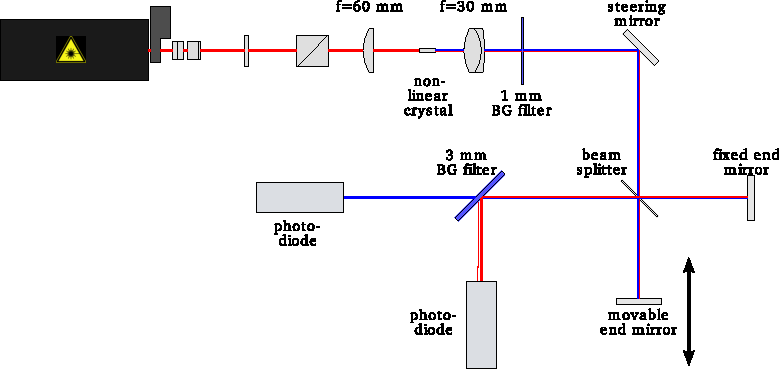
\includegraphics{fig-5}
    \caption{%
        %
    }
    \label{fig:fig-5}
\end{figure}

% TODO Take images of the x-y-mode on the oscilloscope.

% TODO Explain the meaning of the oscillograms.
% TODO Determine deviation from 1:2 ratio.
% TODO What causes the deviation?
% TODO Compare with literature values.
% TODO Compute spectral representation of the interferometer.

\end{document}

% vim: spell spelllang=en_us tw=79
